\documentclass{article}
\usepackage[UTF8]{ctex}
\usepackage[T1]{fontenc}
\usepackage[utf8]{inputenc}
\usepackage{latexsym}
\usepackage{amsmath}
\usepackage{amssymb}
\usepackage[colorlinks, linkcolor = black]{hyperref}
\usepackage{float}
\usepackage[table, xcdraw]{xcolor}
\usepackage{graphicx}
\usepackage{listings}
\lstset{
    basicstyle = \ttfamily,
    keywordstyle = \bfseries,
    commentstyle = \textnormal,
    % linewidth = \linewidth,
    xleftmargin = 0.1\textwidth,
    % xrightmargin = 0pt,
    frame = none,
    escapeinside = ``,
}

\title{Homework 7}
\author{PB17000297 罗晏宸}
\date{May 30 2020}

\begin{document}
\maketitle

\section{Exercise 5.6}
假定图 \ref{5-24} 的缓存内容和和表 \ref{5-12} 中实现方式 1 的定时参数。以下代码序列在基本协议和练习 5.5 的新 MESI 协议中的总停顿周期为多少?假定不需要互连事务的状态转换不会导致额外的停顿周期。
\begin{figure}[h]
    \centering
    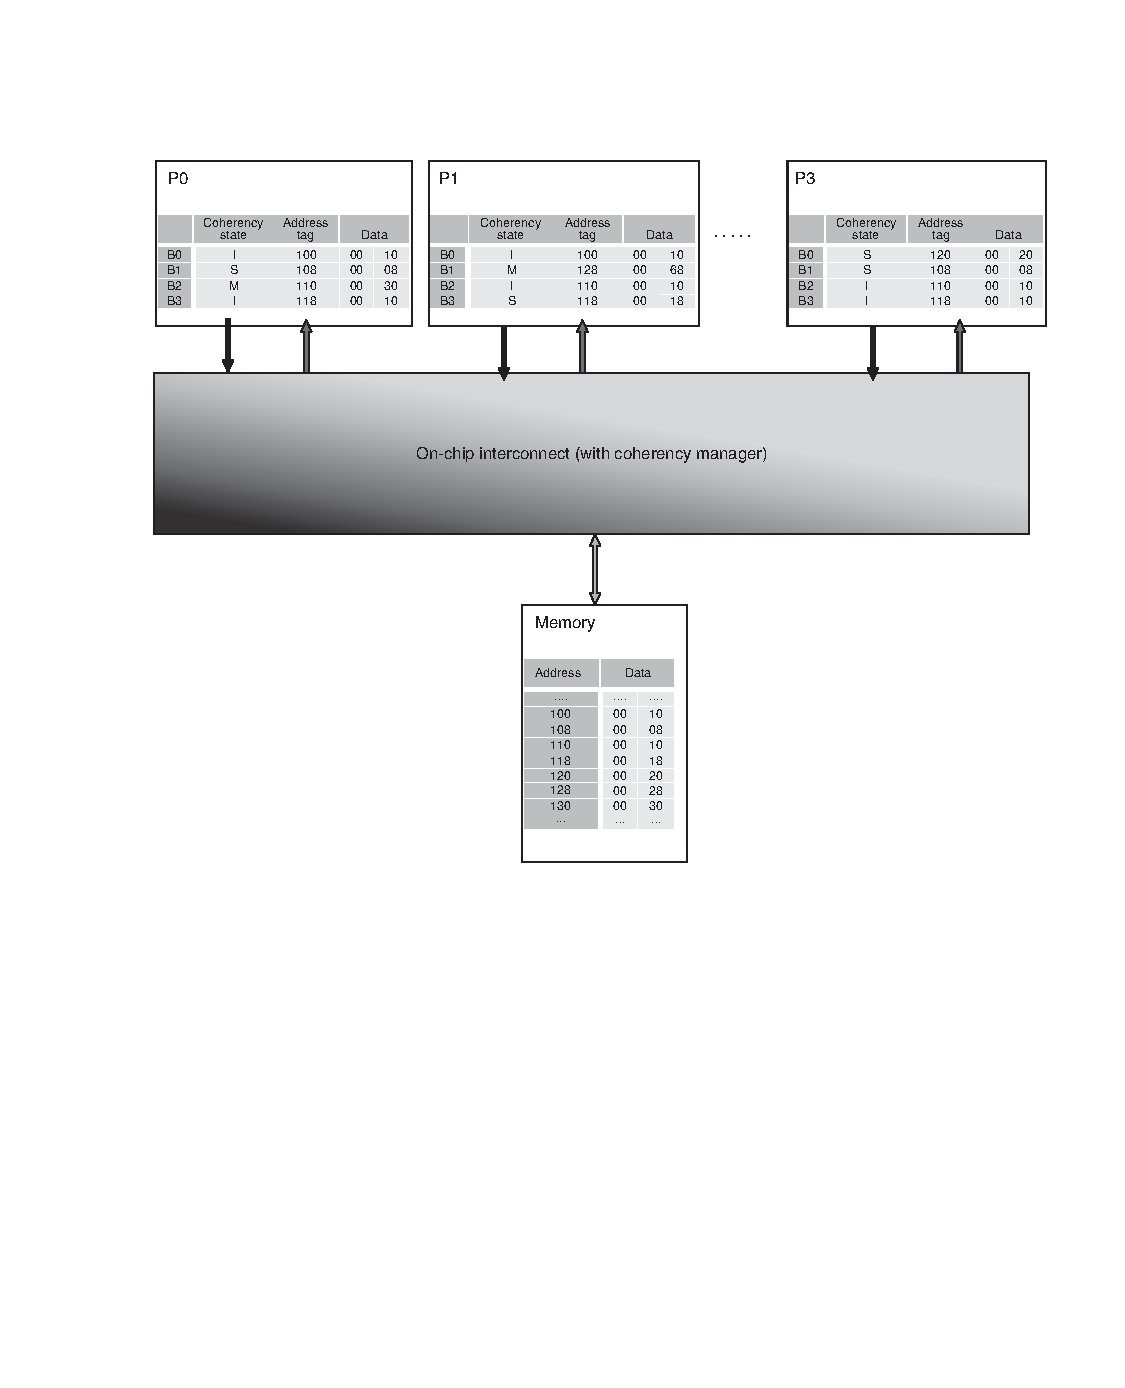
\includegraphics[scale = 0.78]{Figure/5-24.pdf}
    \caption{\textbf{多核(点对点)多处理器}}
    \label{5-24}
\end{figure}
\begin{figure}[h]
    \centering\caption{\textbf{监听一致性延迟}}
    \label{5-12}
    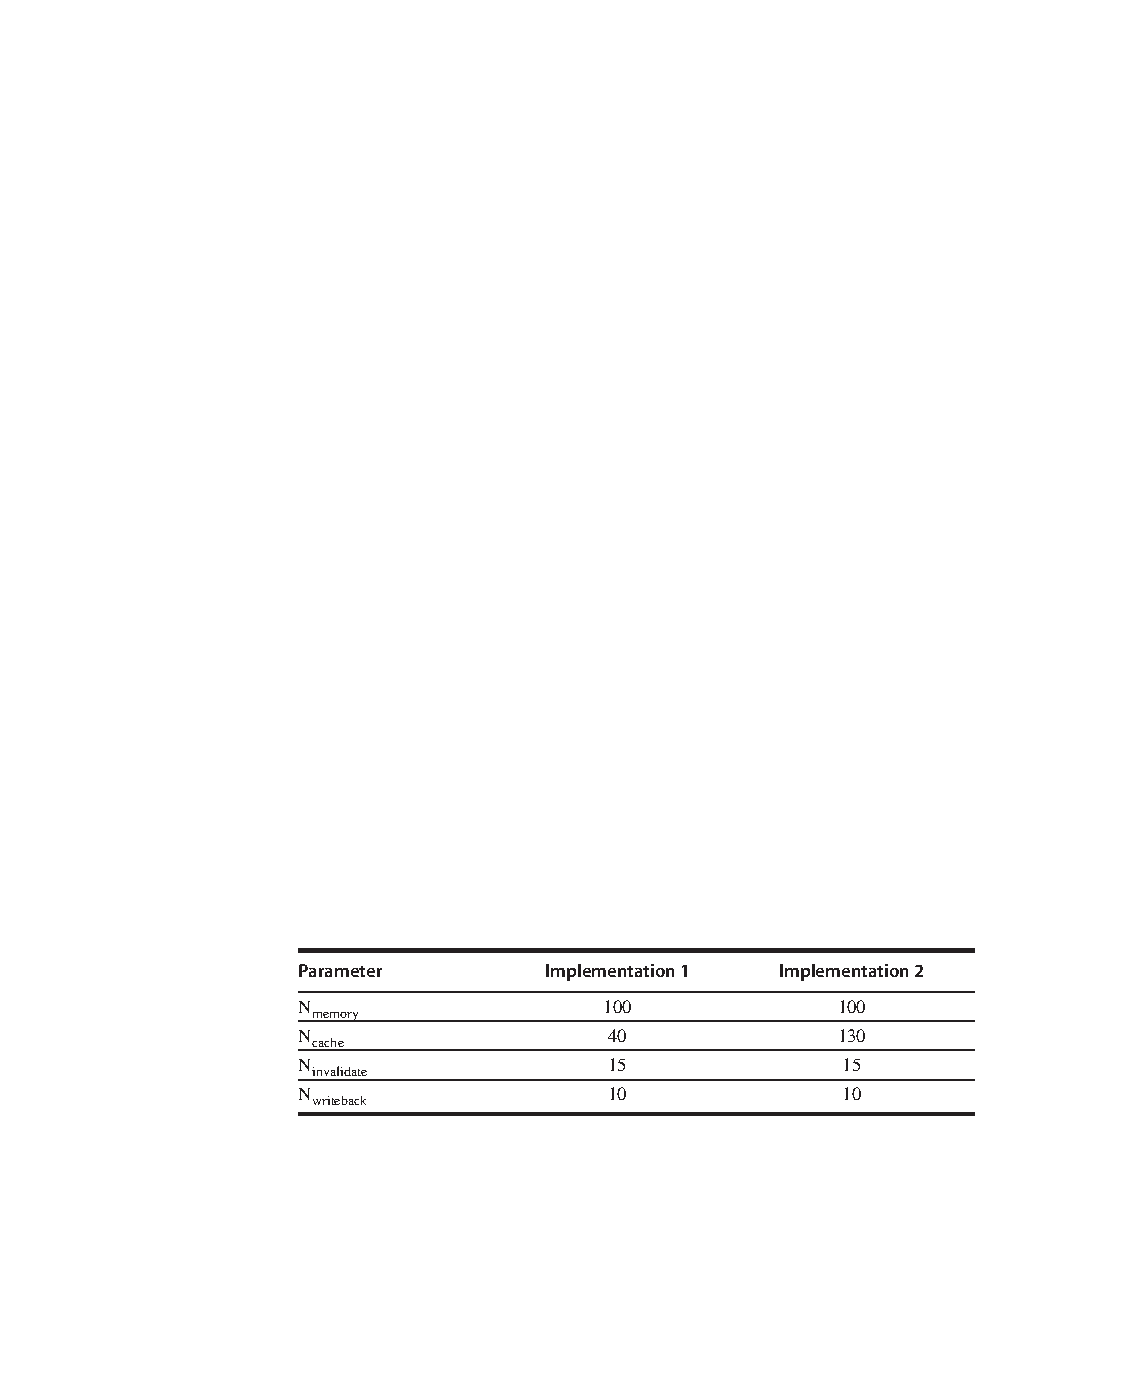
\includegraphics[scale = 1]{Figure/5-12.pdf}
\end{figure}
\subparagraph{a}
\begin{lstlisting}[]
    P0: read 100
    P0: write 100 <-- 40
\end{lstlisting}
\subparagraph{b}
\begin{lstlisting}[]
    P0: read 120
    P0: write 120 <-- 60
\end{lstlisting}
\subparagraph{c}
\begin{lstlisting}[]
    P0: read 100
    P0: read 120
\end{lstlisting}
\subparagraph{d}
\begin{lstlisting}[]
    P0: read 100
    P1: write 100 <-- 60
\end{lstlisting}
\subparagraph{e}
\begin{lstlisting}[]
    P0: read 100
    P0: write 100 <-- 60
    P1: write 100 <-- 40
\end{lstlisting}
\paragraph{解}
\subparagraph{a} \lstinline{P0: read 100} ,发生读缺失,读取内存,停顿 100 个周期,若在 MSI 协议中,则进入状态 S ,若在 MESI 协议中,则进入状态 E ; \lstinline{P0: write 100} ,若在 MSI 协议中,发生写命中,发送失效信号,若在 MESI 协议中,则不发送失效信号,进入状态 M 。

因此 MSI 协议中的总停顿周期
$$
    100 + 15 = 115
$$

MESI 协议中的总停顿周期
$$
    100 + 0 = 100
$$

\subparagraph{b} \lstinline{P0: read 120} ,发生读缺失,读取内存,停顿 100 个周期,在 MSI 协议或 MESI 协议中,均进入状态 S ; \lstinline{P0: write 120} ,在 MSI 协议或 MESI 协议中,均发生写命中,发送失效信号。

因此 MSI 协议与 MESI 协议中的总停顿周期均为
$$
    100 + 15 = 115
$$

\subparagraph{c} \lstinline{P0: read 100} ,发生读缺失,读取内存,停顿 100 个周期,若在 MSI 协议中,则进入状态 S ,若在 MESI 协议中,则进入状态 E ; \lstinline{P0: read 120} ,发生读缺失,读取内存,停顿 100 个周期,在 MSI 协议或 MESI 协议中,均进入状态 S 。

因此 MSI 协议与 MESI 协议中的总停顿周期均为
$$
    100 + 100 = 200
$$

\subparagraph{d} \lstinline{P0: read 100} ,发生读缺失,读取内存,停顿 100 个周期,若在 MSI 协议中,则进入状态 S ,若在 MESI 协议中,则进入状态 E ; \lstinline{P0: write 100} ,发生写缺失,读取内存,停顿 100 个周期,不需要发送失效信号。

因此 MSI 协议与 MESI 协议中的总停顿周期均为
$$
    100 + 100 = 200
$$

\subparagraph{e} \lstinline{P0: read 100} ,发生读缺失,读取内存,停顿 100 个周期,若在 MSI 协议中,则进入状态 S ,若在 MESI 协议中,则进入状态 E ; \lstinline{P0: write 100} ,若在 MSI 协议中,发生写命中,发送失效信号,若在 MESI 协议中,则不发送失效信号,进入状态 M 。 \lstinline{P1: write 100} ,发生写缺失,在 MSI 协议或 MESI 协议中,从 P0 缓存中读取脏块, 再将脏块写回内存。

因此 MSI 协议中的总停顿周期
$$
    100 + 15 + 40 + 10 = 165
$$

MESI 协议中的总停顿周期
$$
    100 + 0 + 40 + 10 = 150
$$

\end{document}